\documentclass[11pt]{article}

\usepackage[margin=1in]{geometry}
\usepackage{graphicx}
\usepackage{amsmath}
\usepackage{amssymb}
\usepackage{booktabs}
\usepackage{array}
\usepackage{float}
\usepackage{hyperref}

\title{Experimental Comparison of 2-bit Vector Quantizers}
\author{Diego Manuel Maldonado Nunez\\Student ID: 202620726}
\date{July 2026}

\begin{document}
\maketitle

\section{Introduction}

Vector quantization is a compression method in which a real-valued vector is represented by an index into a finite codebook. Instead of storing every coordinate of the original vector using full precision, the quantizer maps the vector to one of a limited number of representative vectors, and the dequantizer maps the stored code back to an approximate reconstruction. This is useful when the original vectors are expensive to store or move, but some approximation error is acceptable.

This experiment studies vector quantization in a controlled 24-dimensional setting. Each algorithm receives the same input vectors and is constrained to an effective rate of 2 bits per dimension. The goal is not only to determine which method reconstructs vectors most accurately, but also to determine the practical cost of using each method. For this reason, the experiment evaluates three dependent variables: reconstruction quality, quantization time, and dequantization time.

The three algorithms compared are:

\begin{itemize}
    \item \textbf{Leech Lattice Vector Quantization}: a lattice-based vector quantizer built on the 24-dimensional Leech lattice. The experiment uses 24-dimensional input blocks because the Leech lattice is defined in $\mathbb{R}^{24}$, so each block can be treated as one lattice-quantized vector. This dimension is also mathematically important: the Leech lattice achieves the optimal sphere packing density in 24 dimensions~\cite{sphere24}, and recent Leech Lattice Vector Quantization work uses its symmetry, shell structure, indexing, and search procedures to quantize without materializing a full unstructured codebook~\cite{llvq}. In this experiment, the finite codebook is the union of Leech lattice shells up to shell 13. Shell 13 is used because the cumulative shell count requires 48 index bits, which gives exactly $48/24=2$ bits per dimension.
    \item \textbf{Uniform scalar 2-bit}: a simple coordinate-wise quantizer. Each coordinate is rounded independently to one of a small number of uniformly spaced levels. This method is simple and fast, but it does not use relationships between coordinates.
    \item \textbf{QTIP bitshift}: an additional quantization algorithm based on the bitshift codebook component from QTIP, which stands for Quantization with Trellises and Incoherence Processing~\cite{qtip}. QTIP uses trellis-coded quantization to support very high-dimensional quantization, and introduces a hardware-efficient bitshift trellis for fast decoding.
\end{itemize}

The main research question is:

\begin{quote}
Which 2-bit quantization algorithm gives the best trade-off between reconstruction quality, quantization time, and dequantization time?
\end{quote}

The expected trade-off is that a structured vector quantizer such as Leech Lattice Vector Quantization may achieve better reconstruction quality, while simpler scalar or bitshift methods may run faster.

\section{Experiment Design}

\subsection{Variables}

The independent variable is the quantization algorithm, with three levels: Leech Lattice Vector Quantization, Uniform scalar 2-bit, and QTIP bitshift. The dependent variables are SQNR bits, quantize seconds, and dequantize seconds.

\subsubsection{SQNR bits}

SQNR bits is the signal-to-quantization-noise ratio expressed in bits. Higher is better. This is the quality metric used for sample-size calculation, hypothesis testing, and interpretation. For an original vector $x \in \mathbb{R}^d$ and its dequantized reconstruction $\hat{x} \in \mathbb{R}^d$, SQNR bits measures the ratio between signal power and quantization-noise power, expressed in base-2 logarithmic units:

\[
\mathrm{SQNR}_{\mathrm{bits}}(x,\hat{x}) =
\frac{1}{2}\log_2
\left(
\frac{
\frac{1}{d}\sum_{i=1}^{d}x_i^2
}{
\frac{1}{d}\sum_{i=1}^{d}(x_i-\hat{x}_i)^2
}
\right).
\]

This formulation is useful because it normalizes the reconstruction error by the power of the original vector.

\subsubsection{Quantize seconds}

Quantize seconds is the wall-clock time needed to encode one vector. Lower is better. This measures the cost of producing the compressed representation, which matters when vectors must be encoded online or repeatedly during a larger pipeline.

\subsubsection{Dequantize seconds}

Dequantize seconds is the wall-clock time needed to decode one vector. Lower is better. This measures the cost of reconstructing vectors from their compressed representation, which matters when compressed vectors are read frequently or used in downstream computation.

These three metrics were selected because they correspond to the practical trade-off in a quantization system: reconstruction quality, encoding cost, and decoding cost. Considering them together makes it possible to distinguish an algorithm that is accurate but expensive from one that is faster but less accurate.

\subsection{Hypotheses}

For each metric, the global ANOVA-style hypothesis is:

\[
H_0: \mu_1 = \mu_2 = \mu_3
\]

\[
H_1: \exists i,j \text{ such that } \mu_i \neq \mu_j
\]

For SQNR bits, larger means better reconstruction. For quantization and dequantization time, smaller means better runtime performance.

\section{Data Collection Protocol}

The experiment was implemented in \texttt{quantizer\_sample\_size\_experiment.ipynb}. All input vectors were generated from a standard normal distribution with dimension 24. The random seed was fixed to 0 for repeatability.

The experiment was conducted in two phases:

\begin{enumerate}
    \item \textbf{Pilot experiment}: 30 paired blocks were collected. In each block, the same vector was evaluated by all three algorithms.
    \item \textbf{Final experiment}: the final number of paired blocks was chosen using the pilot-based sample-size calculation described below.
\end{enumerate}

Each block consisted of one vector evaluated by every algorithm. This creates a paired design: all algorithms are compared on the same input vectors. The order of algorithms was randomized during timing to reduce ordering effects. Before timing, each algorithm was warmed up for 5 iterations. For GPU timing, CUDA synchronization was performed before and after each measured call, so asynchronous CUDA execution would not contaminate timing measurements.

Each CSV row records the phase, block id, method, SQNR bits, quantization time, dequantization time, the original vector, the dequantized vector, dimension, and seed. The final data used in this report is:

\begin{center}
\texttt{results/quantizer\_sample\_size\_experiment/seed0\_20260704\_151404/final\_experiment.csv}
\end{center}

\section{Data Analysis Protocol}

First, the pilot data was used to estimate the within-algorithm variance for each metric. A power calculation for a three-algorithm mean comparison was then performed. Two effect scenarios were evaluated:

\begin{itemize}
    \item \textbf{Two levels symmetric}: two algorithms differ symmetrically around the grand mean.
    \item \textbf{One versus rest}: one algorithm differs from the other algorithms.
\end{itemize}

For each metric and scenario, the minimum sample size per algorithm was calculated using the noncentral F distribution. The final experiment used the largest required sample size across all metrics and scenarios. The target significance level was $\alpha = 0.05$ and the desired power was $0.80$.

The minimum interesting differences were:

\begin{itemize}
    \item SQNR bits: 0.10 bits.
    \item Quantize time: 0.001 seconds.
    \item Dequantize time: 0.00005 seconds.
\end{itemize}

After collecting the final data, descriptive statistics were computed for each metric and algorithm, including mean, standard deviation, coefficient of variation, and 95\% confidence intervals. The global tests used were repeated-measures ANOVA and Friedman tests. ANOVA assumptions were checked using Shapiro-Wilk tests on repeated-measures ANOVA residuals, and Fligner-Killeen and Levene tests for equality of variances. Pairwise post-hoc comparisons were performed with Bonferroni correction over all planned metric comparisons.

\subsection{Available Hardware and Software}

The experiment was executed on the following machine:

\begin{itemize}
    \item CPU: AMD Ryzen 9 5950X 16-Core Processor, 16 cores / 32 threads.
    \item RAM: 62 GiB system memory.
    \item GPU: NVIDIA GeForce RTX 3080, 10 GiB VRAM, compute capability 8.6.
    \item NVIDIA driver: 595.80.
    \item Operating system: Linux 7.0.13-200.fc44.x86\_64.
    \item Python: 3.12.9.
    \item PyTorch: 2.12.1+cu130, CUDA 13.0 available.
    \item NumPy: 2.4.6, Pandas: 3.0.3, SciPy: 1.18.0.
\end{itemize}

\section{Actual Experiment}

\subsection{Sample Size Calculation}

Table~\ref{tab:samplesize} shows the pilot-based sample-size calculation. The largest required sample size was 86 observations per algorithm, coming from the SQNR metric under the two-level symmetric scenario. Therefore, the final experiment used 86 paired blocks.

\begin{table}[H]
\centering
\caption{Pilot-based sample-size calculation.}
\label{tab:samplesize}
\begin{tabular}{llrrr}
\toprule
Metric & Scenario & Pilot SD & Min. diff. & Required $n$ \\
\midrule
SQNR bits & Two levels symmetric & 0.209416 & 0.10000 & 86 \\
SQNR bits & One versus rest & 0.209416 & 0.10000 & 65 \\
Quantize seconds & Two levels symmetric & 0.000274 & 0.00100 & 3 \\
Quantize seconds & One versus rest & 0.000274 & 0.00100 & 3 \\
Dequantize seconds & Two levels symmetric & 0.000075 & 0.00005 & 45 \\
Dequantize seconds & One versus rest & 0.000075 & 0.00005 & 34 \\
\bottomrule
\end{tabular}
\end{table}

\subsection{Descriptive Results}

The final experiment collected 86 paired observations for each algorithm. Figure~\ref{fig:boxplots} shows the distributions of the main metrics.

\begin{figure}[H]
\centering
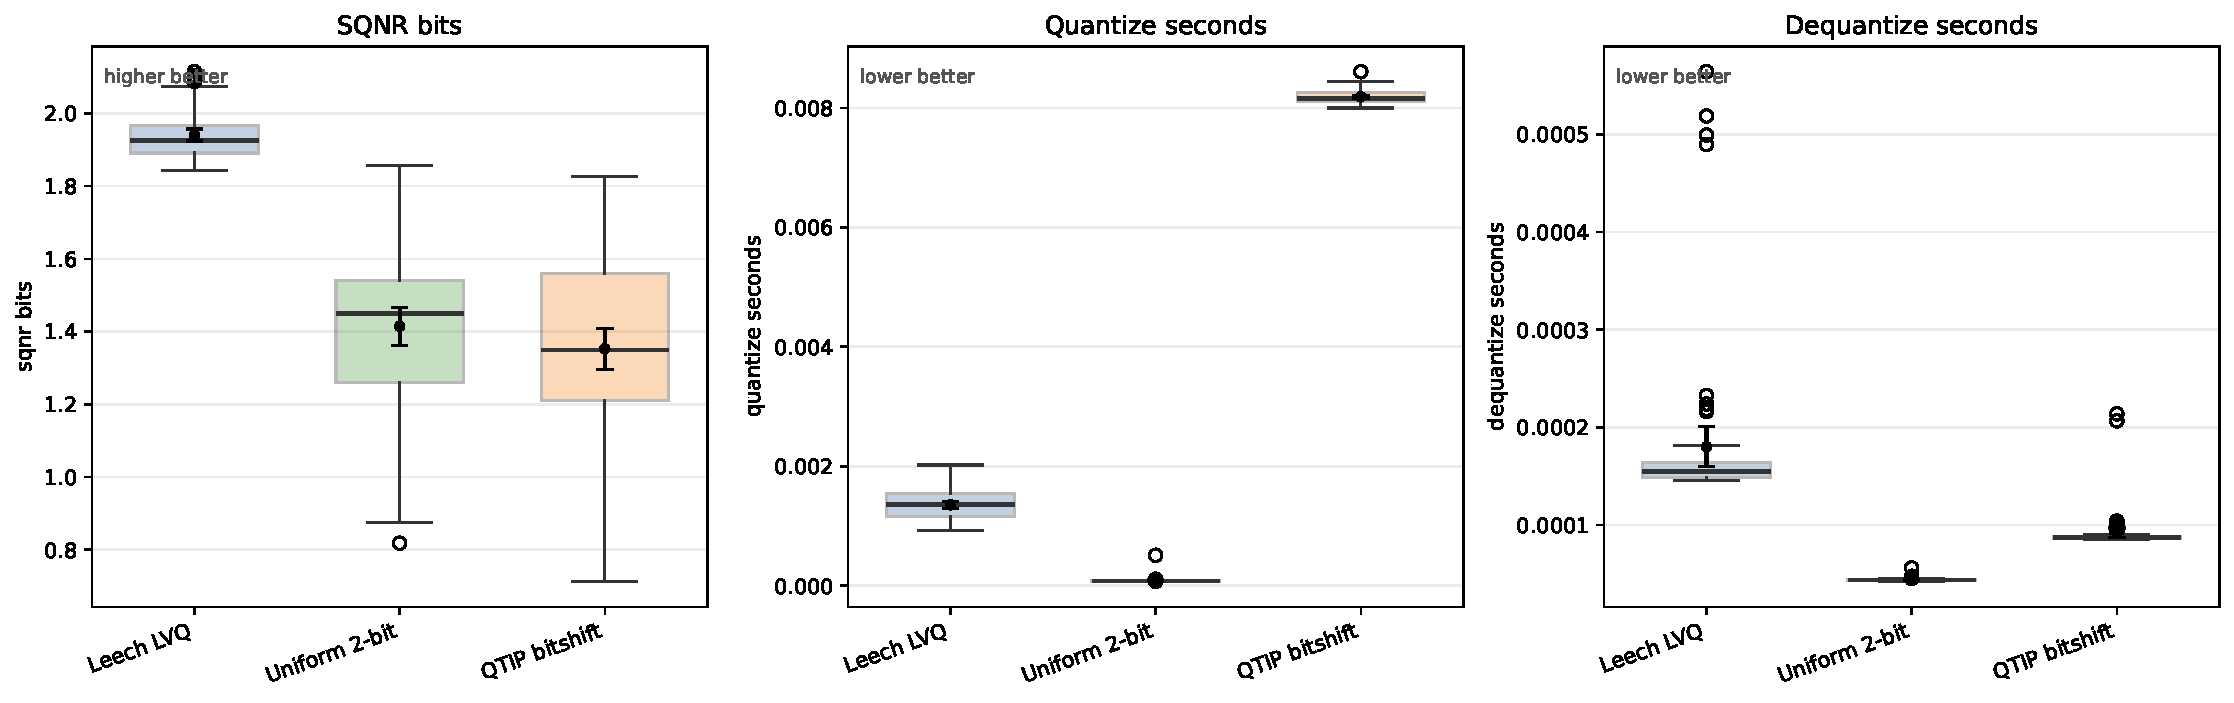
\includegraphics[width=\textwidth]{report_assets/final_metric_boxplots.pdf}
\caption{Final metric distributions for the three algorithms. Black points show the mean with 95\% confidence intervals.}
\label{fig:boxplots}
\end{figure}

Table~\ref{tab:quality} summarizes reconstruction quality. Leech Lattice Vector Quantization achieved the best reconstruction quality, with the highest SQNR bits.

\begin{table}[H]
\centering
\caption{Final reconstruction quality statistics.}
\label{tab:quality}
\resizebox{\textwidth}{!}{%
\begin{tabular}{lrrr}
\toprule
Algorithm & SQNR mean & SQNR 95\% CI & Coef. variation \\
\midrule
Leech Lattice Vector Quantization & 1.855348 & [1.827252, 1.883445] & 0.070632 \\
Uniform scalar 2-bit & 1.477608 & [1.425925, 1.529292] & 0.163143 \\
QTIP bitshift & 1.385363 & [1.336918, 1.433808] & 0.163102 \\
\bottomrule
\end{tabular}
}
\end{table}

Table~\ref{tab:time} summarizes runtime. Uniform scalar quantization was the fastest method for both quantization and dequantization.

\begin{table}[H]
\centering
\caption{Final runtime statistics.}
\label{tab:time}
\resizebox{\textwidth}{!}{%
\begin{tabular}{lrrrr}
\toprule
Algorithm & Quantize mean (s) & Quantize 95\% CI & Dequantize mean (s) & Dequantize 95\% CI \\
\midrule
Uniform scalar 2-bit & 0.000093 & [0.000083, 0.000103] & 0.000047 & [0.000042, 0.000053] \\
Leech Lattice Vector Quantization & 0.001367 & [0.001308, 0.001425] & 0.000202 & [0.000182, 0.000223] \\
QTIP bitshift & 0.008291 & [0.008229, 0.008354] & 0.000096 & [0.000091, 0.000102] \\
\bottomrule
\end{tabular}
}
\end{table}

\subsection{Statistical Tests}

The global tests rejected the null hypothesis for all three primary metrics. Table~\ref{tab:globaltests} shows that both repeated-measures ANOVA and Friedman tests found strong evidence of algorithm differences.

\begin{table}[H]
\centering
\caption{Global statistical tests on final data.}
\label{tab:globaltests}
\begin{tabular}{llrr}
\toprule
Metric & Test & Statistic & p-value \\
\midrule
SQNR bits & Repeated-measures ANOVA & 177.33 & $2.50 \times 10^{-42}$ \\
SQNR bits & Friedman & 118.07 & $2.30 \times 10^{-26}$ \\
Quantize seconds & Repeated-measures ANOVA & 29529.76 & $8.36 \times 10^{-217}$ \\
Quantize seconds & Friedman & 172.00 & $4.47 \times 10^{-38}$ \\
Dequantize seconds & Repeated-measures ANOVA & 158.33 & $1.49 \times 10^{-39}$ \\
Dequantize seconds & Friedman & 164.09 & $2.33 \times 10^{-36}$ \\
\bottomrule
\end{tabular}
\end{table}

The post-hoc comparisons showed the following ordering:

\begin{itemize}
    \item \textbf{SQNR bits}: Leech Lattice Vector Quantization $>$ Uniform $>$ QTIP.
    \item \textbf{Quantize time}: Uniform $<$ Leech Lattice Vector Quantization $<$ QTIP.
    \item \textbf{Dequantize time}: Uniform $<$ QTIP $<$ Leech Lattice Vector Quantization.
\end{itemize}

Every pairwise comparison was significant after Bonferroni correction. The adjusted alpha was 0.005556.

\subsection{Assumption Checks}

Table~\ref{tab:assumptions} summarizes the ANOVA assumption checks. SQNR residuals passed the Shapiro-Wilk normality check, but the timing metrics did not. Equality of variances was rejected for all three metrics. Therefore, the repeated-measures ANOVA results should be interpreted with caution. The Friedman tests are important because they corroborate the same conclusion without relying on normal residuals.

\begin{table}[H]
\centering
\caption{ANOVA assumption checks.}
\label{tab:assumptions}
\begin{tabular}{llrr}
\toprule
Metric & Assumption test & p-value & Passes $\alpha=0.05$ \\
\midrule
SQNR bits & Shapiro-Wilk residual normality & 0.3036 & Yes \\
SQNR bits & Fligner-Killeen equal variances & $7.82 \times 10^{-7}$ & No \\
Quantize seconds & Shapiro-Wilk residual normality & $1.54 \times 10^{-4}$ & No \\
Quantize seconds & Fligner-Killeen equal variances & $2.20 \times 10^{-23}$ & No \\
Dequantize seconds & Shapiro-Wilk residual normality & $2.54 \times 10^{-18}$ & No \\
Dequantize seconds & Fligner-Killeen equal variances & $4.82 \times 10^{-24}$ & No \\
\bottomrule
\end{tabular}
\end{table}

\section{Discussion}

The results show that there is no single best algorithm across all metrics. Leech Lattice Vector Quantization is the best choice when reconstruction quality is the priority. It achieved the highest SQNR. However, this quality comes with higher runtime cost. Uniform scalar quantization was much faster in both quantization and dequantization, but its reconstruction quality was lower. QTIP bitshift was not competitive in this configuration: it had the lowest SQNR and the slowest quantization time among the three algorithms, although its dequantization time was faster than Leech Lattice Vector Quantization.

The assumption checks are an important limitation. The timing data clearly violates normality and equal-variance assumptions, so the repeated-measures ANOVA results for timing should be interpreted cautiously. For this reason, the Friedman test is treated as a robustness check. Since both ANOVA and Friedman agree that the algorithms differ, the main conclusion is stable. However, exact ANOVA p-values for timing metrics should not be over-interpreted.

\section{Conclusion}

This experiment compared three 2-bit quantization algorithms under a controlled paired design. The final sample size was calculated from a pilot study, resulting in 86 paired observations.

Leech Lattice Vector Quantization produced the best reconstruction quality, with SQNR mean 1.855 bits. Uniform scalar quantization was the fastest method, with mean quantization time 0.000093 seconds and mean dequantization time 0.000047 seconds. QTIP bitshift did not dominate either quality or runtime in this experimental configuration.

Therefore, the recommended algorithm depends on the objective. If quality is the priority, Leech Lattice Vector Quantization should be selected. If runtime is the priority, especially for quantization and dequantization latency, the uniform scalar quantizer is preferable. Under these measurements, no algorithm is best simultaneously for SQNR, quantization time, and dequantization time.

\begin{thebibliography}{9}

\bibitem{qtip}
Albert Tseng, Qingyao Sun, David Hou, and Christopher De Sa.
\textit{QTIP: Quantization with Trellises and Incoherence Processing}.
arXiv:2406.11235, 2024.
\url{https://arxiv.org/abs/2406.11235}

\bibitem{llvq}
Tycho F. A. van der Ouderaa, Mart van Baalen, Paul Whatmough, and Markus Nagel.
\textit{Leech Lattice Vector Quantization for Efficient LLM Compression}.
arXiv:2603.11021, 2026.
\url{https://arxiv.org/abs/2603.11021}

\bibitem{sphere24}
Henry Cohn, Abhinav Kumar, Stephen D. Miller, Danylo Radchenko, and Maryna Viazovska.
\textit{The sphere packing problem in dimension 24}.
Annals of Mathematics, 185(3), 2017.
\url{https://annals.math.princeton.edu/2017/185-3/p08}

\end{thebibliography}

\end{document}
